% Chapter Template

\chapter{General Java Concurrency} % Main chapter title

\label{Chapter1} % Change X to a consecutive number; for referencing this chapter elsewhere, use \ref{ChapterX}

%----------------------------------------------------------------------------------------
%	SECTION 1
%----------------------------------------------------------------------------------------

%-----------------------------------
%	SUBSECTION 1
%-----------------------------------
\section{Basic concurrency concepts}
Concurrency and parallelism are similar concepts. Concurrency generally refers to a situation when you have more than one task in a single processor with a single core, and the task scheduler from the operating system level quickly switches between tasks, such they appear as running simultaneosly. Parallelism is when you have more than one task that run simultaneously on a different processor, core inside a processor or even a different computer. Another definition shows that parallelism refers to having different instances of the same task running at the same time over different parts of a data set. \cite{FernandezGonzalez}

%-----------------------------------
%	SUBSECTION 2
%-----------------------------------
\subsection{Syncronization}
Syncronization is defined as the coordination of two or more tasks to get the desired results. It is of two kinds:
\begin{itemize}
\item Control syncronization, when on task depends on another task result
\item Data access syncronization, when multiple tasks have access to a shared variable and only one can access it at any given time
\end{itemize}   

A \textbf{critical section} is a piece of code that is executed by a single task at any time, because it access a shared resource. Mutual exclusion is a mechanism used to make this possible.

From a theoretical point of view, the popular mechanism used to get synchronization in a concurrent system are:
\begin{itemize}
\item Semaphore
\item Monitor
\end{itemize}

A piece of code is thread safe if it can be used in concurrent applications without problems, by using a syncronization mechanism, a nonblocking compare and swap primitive or immutable data. An \textbf{immutable object} is thread-save, because the value of its attributes cannot be modified after initialisation, so you have to create a new one if you want to change it.

An \textbf{atomic operation} is an operation that appers as occcuring simultaneosly to the other tasks, and is implemented using syncronization mechanisms, and an \textbf{atomic variable} is a variable whose value is got and set using atomic operations.

The concurent tasks have two methods to communicate with each other. One is \textbf{shared memory}, and is used when the tasks read and write data from the same memory area, and \textbf{message passing}, used when tasks are running on different computers and nedd to comunicate with each other.

\subsection{Concurrent applications possible problems}

Some of the problems that appear in concurrent applications, caused by the wrong use of syncronization mechanism, are \cite{FernandezGonzalez}:
\begin{itemize}
\item \textbf{Data race (race condition)}, when multiple tasks try to write a shared variable without using any syncronization mechanisms
\item \textbf{Deadlock} occurs when two or more tasks wait for the others to free a shared resource, so they are blocked indefinitely and none will get the resource
\item A \textbf{livelock} occurs when two tasks are always changing their states due to the actions of the other, they are in a loop, unable to continue
\item \textbf{Resource starvation} appears when a task never gets the resource it needs to continue, and \textbf{fairness} is the solution for that problem
\item \textbf{Priority inversion} appears when a resource is holden by a low-priority task and a high-priority task needing it cannot continue its execution
\end{itemize}

\section{Traditional Java Concurrency Model}

\subsection{The Java Thread Model}

Java uses threads to enable its entire environment to be anynchronous, reducing inefficiency by preventing the waste of CPU cycles. This multithreading system is build using the \textbf{Thread} class with its methods and the \textbf{Runnable} interface. A thread of execution is encapsulated in a \textbf{Thread} instance. You have to extend the \textbf{Thread} class or to implement the \textbf{Runnable} interface to create a new thread. Some of the methods defined in the \textbf{Thread} class to help you manage threads are presented in ~\ref{fig:threadMethods} \cite{schildt2014}

\begin{figure}[th]
\centering
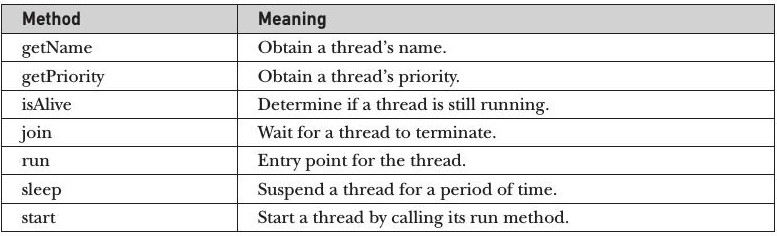
\includegraphics[scale=0.5]{Figures/threadMethods}
\decoRule
\caption{Thread class methods}
\label{fig:threadMethods}
\end{figure}

\subsection{The Main Thread}

A thread begins running when a Java program starts, and it is usually called the main thread. It is used to spawn other child threads and it is the last thread finishing execution and performs some shutdown actions.

\subsection{Creating a thread}

\subparagraph{Implementing Runnable}
To implement Runnable, a class needs to implement only the \textbf{run()} method. Inside this method you define the code that constitues the new thread. The thread will end when run() returns. You have to instantiate a Thread object from within the class that implements Runnable.

\begin{lstlisting}
class NewThread implements Runnable {
  Thread t;

  NewThread() {
    // Create a new, second thread
    t = new Thread(this, "Demo Thread");
    System.out.println("Child thread: " + t);
    t.start(); // Start the thread
  }

  // This is the entry point for the second thread.
  public void run() {
    try {
      for(int i = 5; i > 0; i--) {
        System.out.println("Child Thread: " + i);
        Thread.sleep(500);
      }
    } catch (InterruptedException e) {
      System.out.println("Child interrupted.");
    }
    System.out.println("Exiting child thread.");
  }
}
\end{lstlisting}

\subparagraph{Extending Thread}
Another way to create a thread is to create a class that extends Thread and instantiate it. The entry point of the new thread is the \textbf{run()} method, which has to be overridden. To begin execution of the thread, the new class has to call the start() method.

\begin{lstlisting}
class NewThread extends Thread {

  NewThread() {
    // Create a new, second thread
    super("Demo Thread");
    System.out.println("Child thread: " + this);
    start(); // Start the thread
  }

  // This is the entry point for the second thread.
  public void run() {
    try {
      for(int i = 5; i > 0; i--) {
        System.out.println("Child Thread: " + i);
        Thread.sleep(500);
      }
    } catch (InterruptedException e) {
      System.out.println("Child interrupted.");
    }
    System.out.println("Exiting child thread.");
  }
}
\end{lstlisting}

\subparagraph{isAlive() and join()}

You will often want the main thread to finish last. This can be accomplished by calling sleep(), but the most useful methods are isAlive(), whic returns true if the thread is still alive, or false otherwise, and join(), which waits until the thread on which is called terminates.

\begin{lstlisting}
NewThread ob1 = new NewThread("One");
NewThread ob2 = new NewThread("Two");
NewThread ob3 = new NewThread("Three");
ob1.t.join();
ob2.t.join();
ob3.t.join();
\end{lstlisting}

\subsection{Thread priorities}

The thread scheduler uses thread priorities to decide when a thread should be allowed to run. To set the priority of a thread, we can use the \textbf{setPriority()} method from the Thread class. The values must be in the range \verb|MIN_PRIORITY and MAX_PRIORITY|, currently these values being 1 and 10. The current priority of a thread can be obtained using the \textbf{getPriority()} method.

\section{Syncronization}

\subsection{Using syncronized Methods}

The easiest syncronization method in Java is to use the monitor associated by each object. To enter this monitor, you have to call all method associated with the \textbf{synchronized} keyword. All the other threads that want to call the syncronized method while other thread is inside it have to wait for it to finish.

\subsection{Using syncronized Statement}

To access an object of a class that does not use syncronized methods, you just have to put the calls to that methods inside a syncronized block. The general form of a syncronized block is:
\begin{lstlisting}
syncronized(objRef) {
	//statements to be syncronized
}
\end{lstlisting}

\subsection{Using Syncronization Objects}

To enable handling of several difficult syncronization situations easily, the following syncronization objects are supported: \textbf{Semaphore, CountDownLatch, CyclicBarrier, Exchanger and Phaser}. All these classes are located in the java.util.concurrent package, which defines some core features to support advanced syncronization and interthread communication methods.

\subparagraph{Semaphore}
\subparagraph{CountDownLatch}
\subparagraph{CyclicBarrier}
\subparagraph{Exchanger}
\subparagraph{Phaser}

\section{Using an Executor}

\section{Parallel Programming via the Fork/Join Framework}